
\chapter{Softwares Utilizados}

\section{MikTeX}
O MikTeX é um software para realizar o download dos pacotes utilizadas em qualquer trabalho \TeX. Cada pacote possui uma funcionalidade, seja modificar a fonte do trabalho, permitir a modificação do desing da página ou mesmo a inserção de vídeos, caso esteja a desenvolver um slide.
\subsection{Instalando o MikTeX}
Para instalar o MikTex siga para o site https://miktex.org/, você entrará na área inicial representada na figura \ref{fig_Cap1_siteMikTex}.

\begin{figure}[htb]			
	
	\caption{Tela Inicial do Site MikTeX \label{fig_Cap1_siteMikTex}}
	\begin{center}
		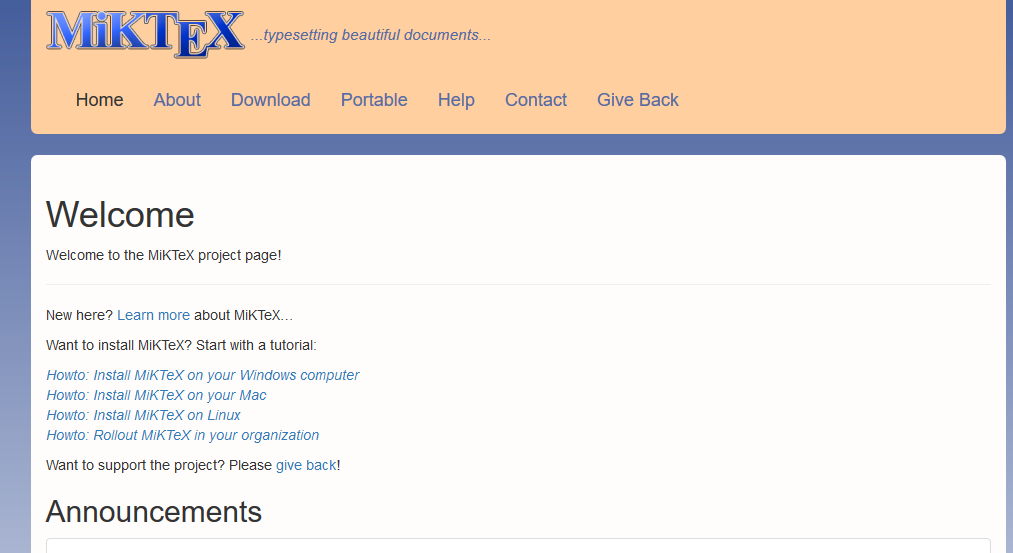
\includegraphics[scale=0.4]{./Imagens/capitulo_1/siteMikTeX.png}
	\end{center}
	\legend{Fonte: https://miktex.org/}
\end{figure}

Após isso vá na seção Downloads escolha o seu sistema operacional, e baixe a ultima versão do software. A versão utilizada neste trabalho foi a v2.9.6515. 

\newpage

\begin{figure}[htb]
	\caption{Área de Download do MikTeX \label{fig_Cap1_downloadMikTex}}
	\begin{center}
		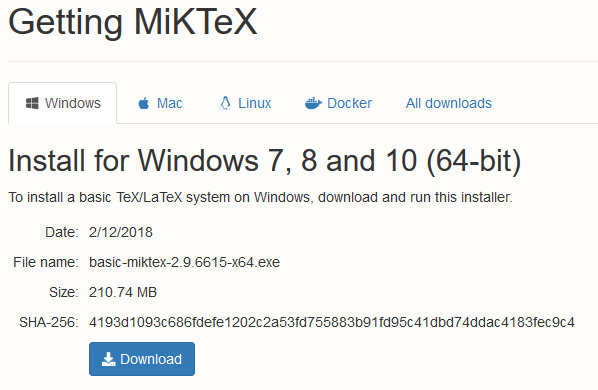
\includegraphics[scale=0.4]{./Imagens/capitulo_1/downloadMikTeX.png}
	\end{center}
	\legend{Fonte: https://miktex.org/}
\end{figure}

Sempre utilize a versão mais atualizada do software, com isto você poderá ter pacotes novos e atualizados, além de muitas correções de erros. Após terminar de realizar o download do software, faça a instalação, e o abra como administrador, a figura \ref{fig_Cap1_MikTeX} representa a forma como é a página inicial do programa.

\begin{figure}[htb]
	\caption{Tela Inicial MikTeX \label{fig_Cap1_MikTeX}}
	\begin{center}
		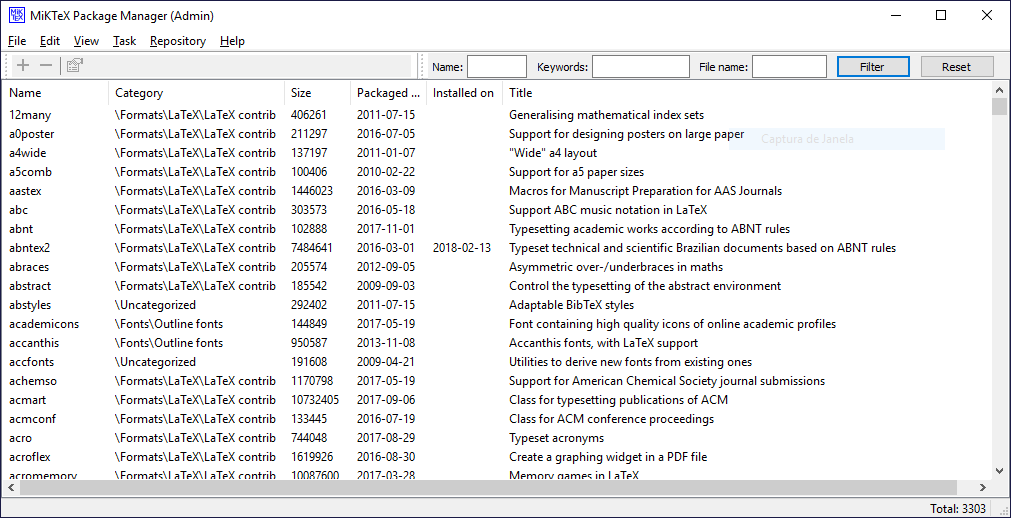
\includegraphics[scale=0.4]{./Imagens/capitulo_1/MikTeX.png}
	\end{center}
	\legend{Fonte: Autoria Própria}
\end{figure}

Aqui é possível baixar a maior parte dos pacotes que será utilizado durante o desenvolvimento do trabalho, mas não é necessário vir neste software para baixar individualmente cada pacote, o próprio programa de tipografia que usaremos já fará isso, este programa é o TeXstudio.

\section{TeXstudio}
O TeXstudio é um software para a escrita de trabalhos no padrão \LaTeX, existem outros softwares no ramo, como por exemplo TeXnicCenter ou TeXMaker, a escolha de qual software utilizar para elaborar o projeto fica a critério do leitor, mas todo este trabalho está sendo elaborado utilizando o TeXstudio, então não há garantias de que todas as funções apresentadas aqui funcionem em outro software.

\subsection{Principais Características do TeXstudio}
O TeXstudio possui diversas características que possibilitam uma facilidade em organizar o código, como a inserção de colores para cada comando, possibilitando uma agilidade na hora de escrever, e corrigir algum erro, e com isso não é necessária tanta atenção ao código, mas sim no texto que se esta escrevendo. O TeXstudio também possibilita a criação de macros, para que agilize no processo de inserção de figuras, tabelas, entre outros.

\subsection{Baixando o Software}
Para realizar o download do software utilizado neste trabalho, o TeXstudio é preciso ir ao site http://texstudio.sourceforge.net/ a figura \ref{fig_Cap1_siteTeXstudio} mostra a tela inicial do site, ao entrar é só clicar em "Download now", assim como o MikTeX, sempre mantenha o software em sua ultima versão, para que não corra riscos de causar algum problema durante o desenvolvimento de seu trabalho.

\begin{figure}[htb]
	\caption{Site TeXstudio \label{fig_Cap1_siteTeXstudio}}
	\begin{center}
		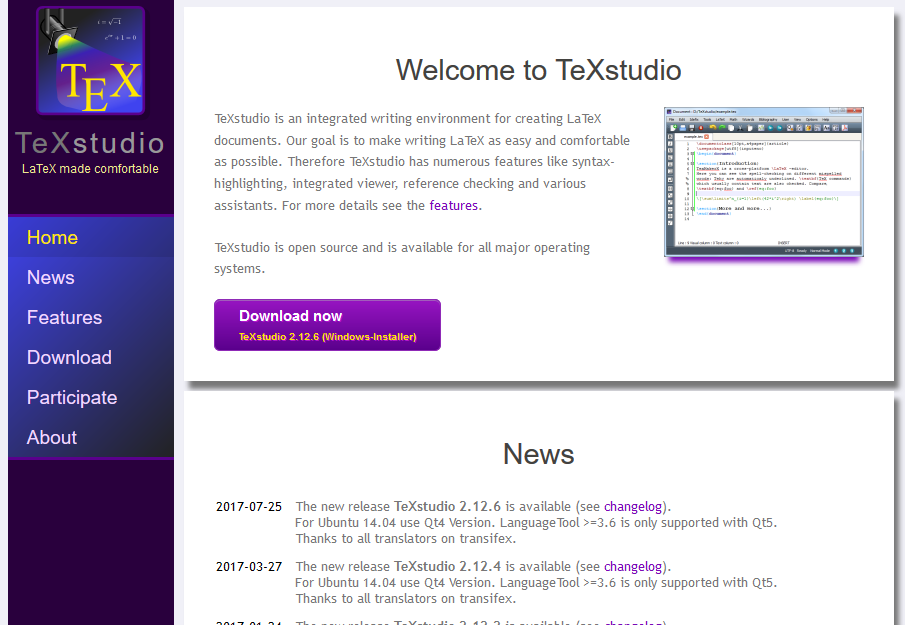
\includegraphics[scale=0.4]{./Imagens/capitulo_1/siteTeXstudio.png}
	\end{center}
	\legend{Fonte: http://texstudio.sourceforge.net}
\end{figure}

Após baixar, instalar o software e abri-lo, você estará na tela inicial, conforme apresentado pela figura \ref{fig_Cap1_TeXstudio}

\begin{figure}[htb]
	\caption{Tela inicial TeXstudio\label{fig_Cap1_TeXstudio}}
	\begin{center}
		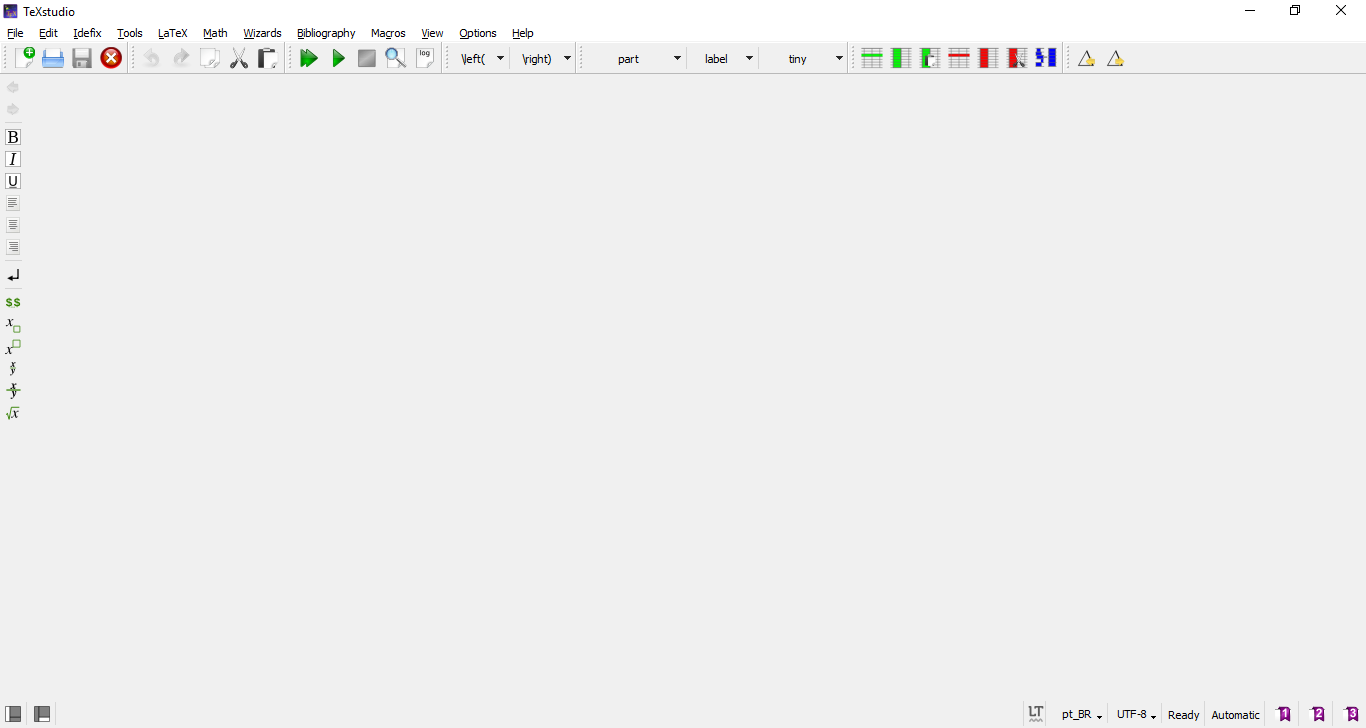
\includegraphics[scale=0.4]{./Imagens/capitulo_1/TeXstudio.png}
	\end{center}
	\legend{Fonte: Autoria Própria}
\end{figure}
\newpage
Com isso, basta ir em ``File'' e ``New'' para criar um projeto em branco, ou em ``File'' e ``Open'' e em seguida abrir o projeto ``modelo.tex'' na página inicial deste trabalho. Com isso, você estará na página principal do trabalho, onde ficam todas as configurações do projeto, para navegar pelos capítulos, entre nas pastas ``elementosPreTextuais'' ou ``elementosTextuais'' e vá até o capitulo que deseje, e abra o arquivo ``.tex'' dentro da pasta. 

OBS: Não feche o arquivo ``modelo.tex'' se não você não conseguira compilar o projeto.

\subsection{Compilando o Projeto}
Após fazer as alterações que deseja, é preciso compilar o trabalho para que seja possível visualizar suas modificações, para isso, pressione a seta dupla no canto superior do software, denominada ``Build \& View'' ou pressione F5. Esteja sempre atento, caso esteja com o arquivo ``modelo.pdf'' aberto, não será possível compilar, para resolver isso, feche o arquivo e compile novamente.